 %\pdfoutput=1
\documentclass[conference]{IEEEtran}
\IEEEoverridecommandlockouts
% The preceding line is only needed to identify funding in the first footnote. If that is unneeded, please comment it out.
\usepackage[T1]{fontenc}
\usepackage{cite}
\usepackage{mathtools}
\usepackage{stackengine}
\def\delequal{\mathrel{\ensurestackMath{\stackon[1pt]{=}{\scriptstyle\Delta}}}}
\usepackage{amsmath,amssymb,amsfonts}
\usepackage{amsmath,epsfig,cite,amsfonts,amssymb,psfrag,subfig}
\usepackage{graphicx}
\usepackage{textcomp}
\usepackage{xcolor}
\usepackage{algorithm}
\usepackage[noend]{algpseudocode}
\usepackage{amsthm}
\def\BibTeX{{\rm B\kern-.05em{\sc i\kern-.025em b}\kern-.08em
    T\kern-.1667em\lower.7ex\hbox{E}\kern-.125emX}}
\allowdisplaybreaks
\newtheorem{remark}{Remark}
\newtheorem{theorem}{Theorem}
\newtheorem{lemma}{Lemma}
\newtheorem{proposition}{Proposition}
\newtheorem{corollary}{Corollary}
\newcommand{\diag}{\mathop{\mathrm{diag}}}
\DeclareMathOperator{\E}{\mathbb{E}}
\usepackage[margin=0.7in]{geometry}
\setlength{\columnsep}{11mm}
\begin{document}

\title{Network Slicing and Resource Allocation in an Open RAN System \vspace{-.1cm}
}
%
%\author{\IEEEauthorblockN{1\textsuperscript{st} Mojdeh Karbalaee Motalleb}
%\IEEEauthorblockA{\textit{Electrical and Computer Engineering} \\
%\textit{Tehran University}\\
%Tehran, Iran \\
%mojdeh.karbalaee@ut.ac.ir}
%\and
%\IEEEauthorblockN{2\textsuperscript{nd} Vahid Shah-Mansouri}
%\IEEEauthorblockA{\textit{Electrical and Computer Engineering} \\
%\textit{Tehran University}\\
%Tehran, Iran \\
%vmansouri@ut.ac.ir}
%\and
%\IEEEauthorblockN{3\textsuperscript{rd} Salar Nouri Naghadeh}
%\IEEEauthorblockA{\textit{Electrical and Computer Engineering} \\
%\textit{Tehran University}\\
%Tehran, Iran \\
%salar.nouri@ut.ac.ir}
%}
%%%%%  \author{
%%%%%    \IEEEauthorblockN{Mojdeh Karbalaee Motalleb}
%%%%%    \IEEEauthorblockA{School of ECE, College of Engineering, University of Tehran, Iran \\
%%%%%    Email: \{mojdeh.karbalaee\}@ut.ac.ir,
%%%%%    \vspace{-.2cm}
%%%%%  }
%%%%%  }

\maketitle

\begin{abstract}

\end{abstract}
\section{Introduction} 

\begin{figure*}
  \centering 
    \includegraphics[scale = 0.5]{finalDraw.pdf}
    %\includegraphics[max height=30cm,max width=9.5cm]{Drawing15.eps}
    %\includegraphics[width=\textwidth]{finalDraw.pdf}
  \caption{Network sliced ORAN system}
  \label{fig:c11}
\end{figure*}



\section{System Model and Problem Formulation}
\subsection{System Model}
%This paper deals with the challenges of heterogeneous vehicular and cellular networks.
Assume we have $S$ preallocated slices serving $S$ services contains eMBB, and URLLC services; We consider $S_1$ slices for the eMBB service type and $S_2$ slices for the URLLC service type. Therefore, we have $S=S_1+S_2$.
Each Service $s\in \{1,2,...,S\} $ consists of $U_{s}$ single-antenna user equipments (UEs) which require certain QoS to be able to use the requested program.
There are different application requests which fall into one of these service categories. Each application request requires specific QoS.
Assume our system consists of $K$, pre-allocated physical resource blocks (PRBs). Moreover, the system  consider to have $M_s^{d}$ VNFs for the processing of O-DU, $M_s^{c}$ VNFs for the processing of O-CU-UP. 
Virtual network functions (VNFs) are functional blocks of the system. Each VNF instance is running on a virtual machine (VM) using resources from the data centers. 
Moreover, we assume the system has $R$ single-antenna O-RU that serverd UEs cooperatively. Each O-RU $r \in \{1,2,...,R \}$ is transmitting and receiving the data of all UEs using the coordinated multipoint transmission (COMP) technology. Moreover, all O-RUs, have access to all PRBs.
\subsection{The Achievable Rate}
The eMBB services typically use more than a one-time slot. But URLLC services use part of a time slot (mini-slot) since it has short packet transmission. In addition, the URLLC must be punctured as soon as it has requested service as it requires very low latency.


The SNR of $i^{th}$ UE requesting  served at slice $s$ is obtained from
\begin{equation}\label{eq2}
\rho_{u(s,i)} =  \frac{\sum_{k=1}^{K_{s}}e_{u(s,i)}^k p_{u(s,i)}^{k}|{\bold{h}_{R,u(s,i)}^{H \: k}}|^2}{BN_0},
\end{equation} 
where $p_{u(s,i)}^{k}$ represents the transmission power allocated by O-RUs to $i^{th}$ UE served at slice $s$ on PRB $k$.
${\bold{h}_{R,u(s,i)}^{k}} \in \mathbb{C}^{R}$ is the vector of channel gain of a wireless link from 
O-RUs to the $i^{th}$ UE in $s^{th}$ slice. 
Moreover, $e_{u(s,i)}^k \in \{0,1\}$ is a binary variable that illustrates whether PRB $k$ is assigned to the $i^{th}$ UE allocated to $s^{th}$ slice or not. 
Also, $BN_0$ denotes the power of Gaussian additive noise.
Moreover, we assume that each PRB is assigned to no more than one UEs. So we have
\begin{equation}
\sum_{s=1}^S \sum_{u=1}^{U_s} e_{u(s,i)}^k = 1
\end{equation} 
The achievable data rate for the $i^{th}$ UE request in the $s_{1}^{th}$ application of service type 1 (eMBB) can be written as $\mathcal{R}_{u(s_1,i)}^{e}$.
\begin{equation}\label{eq1}
\mathcal{R}_{u(s_1,i)} =  B \log_2({1+ \rho_{r,u(s_1,i)}}),
\end{equation}
where $B$ is the bandwidth of system. 
$\mathcal{R}_{u(s_1,i)}^{e,r}$ is the achievable rate of each RU $r$ to UE $i$ in slice $s_1$.
Since the blocklength in URLLC and mMTC is finite, the achievable data rate for the $i^{th}$ UE request in the $s_{2}^{th} $, application of service type 2 (URLLC) is not achieved from Shannon Capacity formula. So, for the short packet transmission the achievable data rate is approximated as follow
\begin{equation}\label{eq11}
\mathcal{R}_{u(s_2,i)}^{\mathfrak{u}} =  B (\log_2({1+ \rho_{u(s_2,i)}})- \zeta_{u(s_2,i)}), 
\end{equation}
where $\zeta_{u(s_2,i)} = \log_2({e})Q^{-1}(\epsilon) \sqrt{\frac{C_{u(s_2,i)}}{N_{u(s_2,i)}}})$
where $\epsilon$ is the transmission error probability, $Q^{-1}$ is the inverse of Q function (i.e., Gaussian),
$C_{u(s_2,i)} = 1 - \frac{1}{(1+\rho_{u(s_2,i)})^2}$ depicts the channel dispersion of UE  $i$ at slice $s_2$, experiencing PRB $k$ and
$N_{u(s_2,i)}$ represents the blocklength of it. 
$\mathcal{R}_{u(s_1,i)}^{e,r}$ is the achievable rate of each RU $r$ to UE $i$ in slice $s_2$.
\subsection{Mean Delay}
In this part, the mean processing delay for each service is obtained.
Suppose the mean processing delay is depicted as $T_{\text{\text{proc}}}$,
\begin{equation}
T^{\text{\text{proc}}} =  T^{RU} + T^{DU} + T^{CU},
\end{equation}
Assume the packet arrival of UEs follows a Poisson process with arrival rate $\lambda_{u(s,i)}$ for the $i^{th}$ UE of the $s^{th}$ service (or slice).
Therefore, the mean arrival data rate of the $s^{th}$ slice in the UPF layer is $\alpha_{s}^U = \sum_{u=1}^{U_s}\lambda_{u(s,i)}$.
Assume the mean arrival data rate for each slice $s$ ($\alpha_{s}$) is approximately equal to the mean arrival data rate of the O-CU-UP layer ($\alpha_{s}^C$) and the O-DU ($\alpha_{s}^D$). so $\alpha_{s} \approx \alpha_{s}^C \approx \alpha_{s}^D$,
Because the amount of data traffic transferred along the route (regardless of frame changes) is constant.
Since, by using Burke’s theorem, the mean arrival data rate of the second and third layers, which are processed in the first layer, is still poisson with rate $\alpha_{s}$.
It is assumed that there are load balancers in each layer for each service to divide the incoming traffic to VNFs equally. %\cite{frdl,luong2018novel,luong2018novel1}.
Suppose the baseband processing of each VNF is depicted as M/M/1 processing queue.
Each packet is processed by one of the VNFs of a slice. So, the mean delay for the $s^{th}$ slice in the O-DU, the O-CU, and the UPF is modeled as M/M/1 queue, is formulated as follows, respectively \cite{SystemCostMinimization,luong2018joint,luong2018novel},
\begin{equation}
\begin{split}
T_{s}^{DU} &= \frac{1}{\mu_s^d - \alpha_{s}/{M_s^{d}}},\\
T_{s}^{CU} &= \frac{1}{\mu_s^c - \alpha_{s}/{M_s^{c}}},\\
\end{split}
\end{equation}
where $M_s^{d}$, $M_s^{c}$ and 
$M_s^{u}$ are the variables that depict the number of VNFs in O-DU, O-CU-UP and UPF, respectively. 
Moreover, $1/\mu_s^d$, and $1/\mu_s^c$ are the mean service time of the O-DU, and O-CU layers, respectively.
Besides, $\alpha_{s}$ is the  arrival rate which is divided
by load balancer before arriving to the VNFs. The arrival rate of each VNF in each layer for each slice 
$s$ is $\alpha_{s}/{M_s^{i}}$ $ i \in \{d,c\}$.

$T_{u(s,i)}^{RU}$ is the mean transmission delay of the $i^{th}$ UE of the $s^{th}$ service on the wireless link.
 The arrival data rate of wireless link for each UE $i$ of service $s$ is $\lambda_{u(s,i)}$
As a result, we have $\sum_{i = 1}^{U_s} \lambda_{u(s,i)} = \alpha_s$.
Moreover, The service time of transmission queue for UE $i$ requesting service $s$ has
an exponential distribution with mean $1/R_{u(s,i)}$ and can be modeled as a M/M/1 queue \cite{SystemCostMinimization,luong2018joint,luong2018novel}.
 
Therefore, the mean delay of the transmission layer for UE $i$ in slice $s$ is
\begin{equation}
 T_{u(s,i)}^{RU} = \frac{1}{R_{u(s,i)} - \lambda_{u(s,i)}}.
\end{equation}

\subsection{Reliability of URLLC}
As we know, UEs request URLLC services, require services with low latency.
For the M/M/1 system, the probability of the delay for each application $s_2$ in the O-RU is as follow, 
\begin{equation}
P_r\{T_{RU}^{s} \geq T_{RU}^{max}\} = e^{-(R_{{tot}_s} - \alpha_{s})T_{RU}^{max}}
\end{equation} 
Also, we do not consider the reliability for O-CU and O-DU.
\subsection{Physical Data Center Resource}
Each VNF requires
physical resources that include memory, and CPU.
Let the required resources for VNF $f$ in slice $s$ is represented by a tuple as
\begin{equation}
\bar{\Omega}_{s}^f = \{\Omega_{M,{s}}^f, \Omega_{C,{s}}^f \},
\end{equation}
where $\bar{\Omega}_{s}^f\in \mathbb{C}^{2}$ and $\Omega_{M,{s}}^f, \Omega_{C,{s}}^f$ indicate the amount of required memory, and CPU, respectively.
Moreover, the total amount of required memory, storage, CPU and Network Bandwidth of all VNFs of a slice in O-DU, and O-CU is defined respectively as follows
\begin{equation}
\begin{split}
&\bar{\Omega}_{\mathfrak{z},s}^{tot,d} = \sum_{f=1}^{M_{s}^d}\bar{\Omega}_{\mathfrak{z},s}^{f,d},\\
&\bar{\Omega}_{\mathfrak{z},s}^{tot,c} = \sum_{f=1}^{M_{s}^c}\bar{\Omega}_{\mathfrak{z},s}^{f,c},\\
\end{split}
\end{equation}
$\forall \mathfrak{z} \in \{M, C\}$, where, $\bar{\Omega}_{\mathfrak{z},s}^{f,d}$, and $\bar{\Omega}_{\mathfrak{z},s}^{f,c}$ are the amount of resource that a VNF required in O-DU, and O-CU, respectively. Then,
\begin{equation}
 \bar{\Omega}_{\mathfrak{z},s}^{tot} = \bar{\Omega}_{\mathfrak{z},s}^{tot,d}+ \bar{\Omega}_{\mathfrak{z},s}^{tot,c}
\end{equation} 
Also, there are $D_c$ data centers (DC), serving the VNFs. Each DC contains several servers that supply VNF requirements.
The amount of memory, and CPU is denoted by $\tau_{M_{j}}$, and $\tau_{C_{j}} $ for the $j^{th}$ DC, respectively
\begin{equation*}
\tau_j = \{\tau_{M_{j}}, \tau_{C_{j}} \},
\end{equation*}
In this system model, the assignment of physical DC resources to VNFs is considered. Let $y_{s,d}$ be a binary variable indicating whether the $d^{th}$ DC is allocated the resources to the VNFs of $s^{th}$ slice or not.
\subsection{Problem Statement}
%In this system, the goal is to minimize the cost of the system.
%The total power cost of O-RUs for transmitting data to UE is depicted as follow
%\begin{equation}
%P_{tot} = \sum_{r=1}^{R}P_r
%\end{equation}
Assume the power consumption of baseband processing at each DC $d$ that is connected to VNFs of a slice $s$ is depicted as
$\phi_{s}$. So the total power of the system for all active DCs that are connected to slices can be represented as
\begin{equation*}
\textstyle \phi_{tot} = \sum_{s=1}^{S}\phi_{s} + \sum_{d=1}^{D_c}z_d \psi_d .
\end{equation*}
where, $z_d$ is shown that whether the $d^{th}$ DC is active or not and $\psi_d$ is a static cost when a DC is active, i.e.,
\begin{equation}
  z_d =
    \begin{cases}
      1 & \sum_{s=1}^{S}y_{s,d} \geq 1 \\
      0 & \text{otherwise}
    \end{cases}       
\end{equation}  
Here, we assume that if any VNF placed in a server $d$ is used, the server is on and active, otherwise, it is off.
In addition, $\phi_{s}$ is obtained from below
\begin{equation}
\phi_{s} = M_s^u \phi_s^u + M_s^c \phi_s^c+ M_s^d \phi_s^d
\end{equation}
where, $\phi_s^u$, $\phi_s^c$ and $\phi_s^d$ are the static cost of energy in UPF, CU and DU, respectively.
Here, we want to maximize the energy efficiency $\eta$. 
So the optimization problem is formulated as follow

\begin{subequations} \label{mainP}
\begin{alignat}{4}
\max\limits_{ \boldsymbol{M}, \boldsymbol{Y}, \boldsymbol{E},\boldsymbol{P},\boldsymbol{G} } &\eta = \frac{\sum_{s=1}^{S_1}\sum_{i=1}^{U_s}R_{u_{(s,k)}}}{\phi_{tot} +P_r}       \ \\
\text{subject to} \quad  & \mathcal{R}_{u_{(s,i)}} \geq  \mathcal{R}_{min}^{s} \quad \forall s, \label{c13} \\
 &\mathcal{R}_{u_{(s,i)}} \leq  \mathcal{R}_{max}^{s} \quad \forall s, \label{c13-1} \\
 &\textstyle \sum_{s=1}^{S} y_{s,d} \bar{\Omega}_{\mathfrak{z},s}^{tot}  \leq   \tau_{\mathfrak{z}_d}, \quad  \mathcal{E} = \{M,C\}, \label{c14}\\
&p_{u(s,i)}^{k}  \geq 0  \quad \forall i,\forall r,\forall s, \forall k,\label{c12} \\
&p_{u(s,i)}^{k}  \leq P_{s}^{max}  \quad \forall i,\forall r,\forall s, \forall k,\label{c12-1} \\
%&\mathcal{R}_{u_{(s_2,i)}}^u \geq  \mathcal{R}_{min}^{s_2,u} \quad \forall s_2, \label{c14} \\
&T^{\text{\text{proc}}}_{u(s,i)}  \leq T^{max}_{s} \quad \forall i,\forall s,\label{c16} \\
& \mu_s \geq \alpha_s/M_s \quad \forall s,\label{c16-1} \\
& \mathcal{R}_{u_{(s,i)}} \geq {\lambda}_{u_{(s,i)}} \quad \forall i,\forall s,\label{c16-2} \\
& 0 \leq M_s \leq M^{max}_s  \quad \forall s,\label{c16-3}\\
%& P_r\{E_1, E_2, E_3, E_4\} \leq \epsilon_s \quad \forall s_2, \label{c166}\\
& \sum_{s =1}^{S}\sum_{i=1}^{U_s} e^{k}_{u(s,i)} = 1  \quad \forall s,\forall i ,\forall r \label{c18} \\
& \phi^{\text{\text{tot}}}  \leq \phi^{max}, \label{c19} \\
& e^k_{r,u(s,i)} \in \{0,1\} \quad \forall s,\forall i, \label{c21}\\  
& P_r\{T_{RU}^{s_2} \geq T_{RU}^{max}\} = e^{-(R_{{tot}_{s_2}} - \alpha_{s_2})T_{RU}^{max}}\label{c22-3}
\end{alignat}
\label{constraints}
\end{subequations}
\noindent where $\boldsymbol{P} =[p_{u(s,i)}^{k}], \:\: \forall s , \forall i,  \forall k $, is the matrix of power for UEs, $\boldsymbol{E} =[e_{u(s,i)}^k], \:\: \forall s , \forall i,  \forall k$ indicate the binary variable for PRB association. Furthermore, $M = [M_s^d, M_s^c], \:\: \forall s$ is the matrix that shows the number of VNFs in each layer of slice.
Also $\boldsymbol{Y} =[y_{s,d}]  \:\: \forall s ,  \forall d $ is a binary variable shown whether
the physical DC is mapped to a VNFs of a slice or not.
\eqref{c12} and \eqref{c12-1} indicate that the power of each UE is a positive integer value, and the power of each UE in each service does not exceed the maximum power of each service, respectively.  
Also, \eqref{c13} and \eqref{c13-1} shows that the rate of each UE requesting each type of service, i.e., eMBB, and URLLC, has a maximum and minimum, respectively.
In addition, in \eqref{c14}, the constraint supports that we have enough physical resources for VNFs of each slice.
\eqref{c16} expressed the limited end-to-end delay of the received signal, respectively.
\eqref{c16-1} and \eqref{c16-2} denoted the stability of the M/M/1 queue model.
\eqref{c16-3} restricted the number of VNF in each slice due to the limited resources.
%\eqref{c16} is a reliability condition that the delay in each layer should be less than the threshold.
\eqref{c18} shows that each PRB are associated to no more than one UE.
In addition, \eqref{c19} indicates that the fixed cost of energy of VNFs in each slice does not exceed the threshold. 
Moreover, \eqref{c21} depicts that $\boldsymbol{E}$ is a matrix of binary variables.
Also, \eqref{c22-3}, guarantees the reliability of the URLLC services.
\subsection{Proposed Algorithm and Numerical Results}
Problem \eqref{mainP}, is a two-time scale problem, i.e., large time scale and small time scale. On a large-time scale, we aim to minimize the power of servers and obtain the QoS of slices. The assignment of PRB to slices is implemented in this time scale. In the small-time scale, the assignment of PRB of slices to UEs is executed, and the optimal power is obtained.
In this research, we aim to use the machine learning methods such as deep reinforcement learning and deep learning to train the O-RAN system and have an intelligent system.
The deep Q-learning is implemented for the large-time scale and 
 the multi-agent deep reinforcement learning contains DDPG (actor-critic algorithm), correlated q-learning, and the priority proportional fairness algorithm will be implemented for the small-time scale. 
The deep learning algorithms contain LSTM and recurrent neural networks.
The proposed algorithm for the large-time scale is implemented in the following, and part of the numerical results is depicted.
\subsubsection{Proposed Algorithm}
Here we use the reinforcement learning method to solve the above two problems.
In the Q-learning method for the large-time scale, an agent tries to find the optimal value in a specific environment. This interactive process is modeled as a Markov decision-making process that includes $ (S, A, R, P, \gamma) $.
S represents the state space matrix, and A represents the action vector. R is also the reward of action. $ P (. | S, a) $ is the probability of transfer and $ \gamma \in (0,1] $ is the discount factor.  The $ \Pi (. | S) $ policy is a mapping of the state to the distribution of actions. The value-state function for state s under policy $ \Pi (. | S) $ with $ V^{\Pi} (s) $ indicates that the expected return value in state s under policy $ \Pi (. | S) ) $. The value of performing operation a in state s under the $ \Pi (. | S) $ policy is represented by $ Q ^ {\Pi} (s, a) $. We have the following relations on this basis.
\begin{equation}
	V^{\Pi}(s) = \mathbb{E}_{\Pi,P}[\sum_{t=0}^{\infty}\gamma^tR_t|S_0=s]
 \end{equation}
 The Q-value is as below.
 \begin{equation}
	Q^{\Pi}(s,a) = \mathbb{E}_{\Pi,P}[\sum_{t=0}^{\infty}\gamma^tR_t|S_0=s,A_0=a].
\end{equation}
 
  $\mathbb{E}$ represented the statistical average. 
 Based on the Bellman equation we have
 \begin{equation}
	V^{\Pi}(s) = \mathbb{E}_{\Pi,P}[R+\gamma V^{\Pi}(s')]
\end{equation}  
 and also, 
   \begin{equation}
  	Q^{\Pi}(s,a) = \mathbb{E}_{\Pi,P}[R+\gamma Q^{\Pi}(s',a')]
  \end{equation}  
  where, $s'$ and $a'$ can be obtained from $\Pi(.|s')$ and $P(.|s,a)$.
The goal of reinforcement learnin is to obtain the optimal policy to maximize the $Q^{\Pi}(s,a)$.
So, using Bellman equation, we have
\begin{equation}
	Q^{*}(s,a) = \mathbb{E}_{\Pi^*,P}[R+\gamma Q^{*}(s',a')].
\end{equation} 
Also, $T^*$ is the Bellman operator
\begin{equation}
	T^{*}Q(s,a) = \mathbb{E}_{\Pi^*,P}[R+\gamma Q(s',a')]
\end{equation} 
By using this operator iteratively, 
$Q_{t+1}(s,a) \leftarrow T^{*}Q(s,a) $
the algorithm can converge
$Q_{t}(s,a) \rightarrow Q^*(s,a)$.
 $t \rightarrow \infty $
\cite{montague1999reinforcement,gan1}.
In the Q-learning in each episode we have
\begin{equation}
	Q(s_{t+1},a_{t+1}) = Q(s_t,a_t)+\alpha[ r_{t+1} + \gamma \max_{a \in A}{Q(s_{t+1},a)}-Q(s_t,a_t)]
\end{equation}
where, $\alpha$ is the learning rate.

\bibliographystyle{IEEEtran}
\bibliography{ref}
\end{document} 